
\documentclass{article}
\usepackage{amsmath}
\usepackage[utf8]{inputenc}
\usepackage{ctex}
\usepackage{indentfirst}

\usepackage{graphicx}

\usepackage{listings}
\usepackage{color}

\lstset{
    language=Python, % 设置语言
    basicstyle=\ttfamily, % 基本字体样式
    keywordstyle=\color{blue}, % 关键词的颜色
    commentstyle=\color{green}, % 注释的颜色
    stringstyle=\color{red}, % 字符串的颜色
    showstringspaces=false, % 不显示字符串间隙
    numbers=left, % 显示行号
    numberstyle=\tiny\color{gray}, % 行号样式
    breaklines=true, % 自动换行
    frame=single % 给代码框加一个边框
}


\setlength{\parindent}{2em}

\begin{document}

\begin{center}
    \Large \textbf{Lab5 实验报告}\\
    \vspace{1em}
    姓名:~~学号:~~班级:
\end{center}

\section{实验概览}

    本次实验学习了简单的机器学习和深度学习知识。通过pytorch构建了自己的网络实现图像分类和图像检索。

    机器学习的本质是找到一个函数,使得对给定的输入有一个令人满意的输出。

    由于我们求解的函数通常有着多维输入和输出,求解这个函数的过程通常采用神经网络方法。

\begin{figure}[h]
\centering
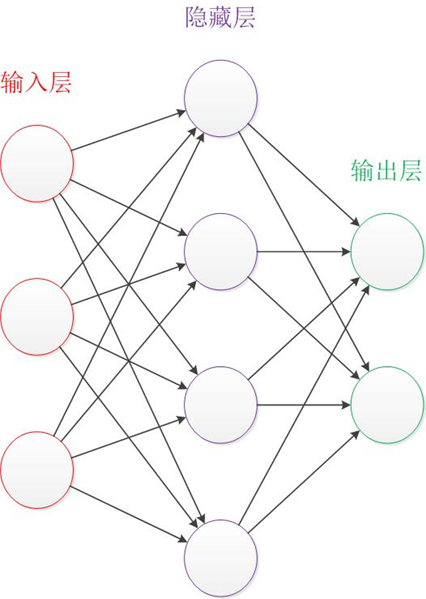
\includegraphics[width=0.6\textwidth]{figure/img1}
\caption{神经网络}
\end{figure}

    这是一个包含三个层次的神经网络。红色的是输入层,绿色的是输出层,紫色的是中间层(也叫隐藏层)。
    输入层有3个输入单元,隐藏层有4个单元,输出层有2个单元。
    后文中,我们统一使用这种颜色来表达神经网络的结构。

    通常情况下,输入和输出的单元是固定的,而隐藏层的单元数可以手动调节。
    求解神经网络的过程就是求解层与层之间单元的函数关系,进而拟合出总体的输入和输出的关系。
    可以视为一种加权求和。

    当然,可以有多个隐藏层。现代神经网络通常有几十层或者更多,对于这种多层神经网络的训练,可以认为是深度学习。

    神经网络的训练通常包括前向传播(得到输出结果),计算损失(输出结果和期望结果的误差),
    反向传播(根据误差,通过梯度下降等方法改变网络中间的权值,以期望得到更好的结果),更新权重等过程。

\section{练习题的解决思路}

\subsection{1.CIFAR-10图片分类}

    exp2.py中的test函数需要我们完善。注意到这里是test部分,我们不需要更新权重,只需要通过前向传播
    得到输出结果即可。通过统计每个batch中匹配的数量和batch的大小即可计算正确率,代码如下:

\begin{figure}[h]
\centering
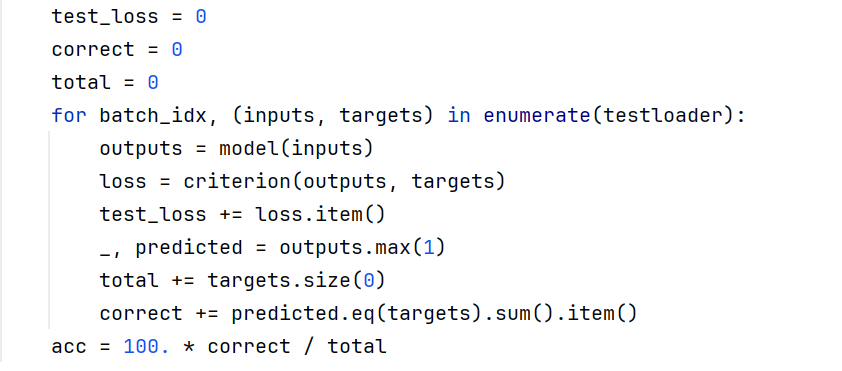
\includegraphics[width=0.6\textwidth]{figure/prog_1}
\caption{代码片段1}
\end{figure}

    对于自动训练(即前五个epoch的lr设置为0.1,后五个设置为0.01)只需要在第六个epoch训练开始前将lr更新,
    并修改optimizer中的lr信息即可。参考如下:

\begin{figure}[h]
\centering
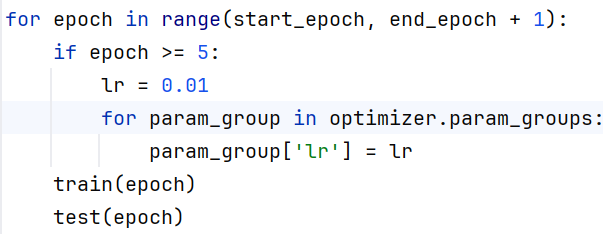
\includegraphics[width=0.6\textwidth]{figure/prog_2}
\caption{代码片段1}
\end{figure}

    对于可视化部分,主要使用了tensorboard库自带的训练可视化功能,通过
    将训练过程中的loss和acc等数据写入指定的文件夹,再通过tensorboard --logdir=dir
    (dir为指定的目录)在本机生成对应的web网页,将数据可视化。

\subsection{2.图像特征提取}

    类似于lab4中的LSH操作,我们需要从图像中提取特征信息。只不过与LSH操作不同的是,
    我们将整个图像的每个像素点都直接作为输入,通过一系列操作,得到远多于LSH操作的特征信息。

    本次实验仍采用了推荐的ResNet50作为神经网络的模型,包含一系列的卷积、降采样、池化等操作,
    可以将\(1 \times 3 \times 224 \times 224\)的输入映射到\(1 \times 2048 \times 1 \times 1\)的特征向量上。
    具体细节不过多赘述。

    将特征向量resize成size为2048的向量,再通过除以向量的模长(L2-norm)进行归一化,即可通过简单的点积操作
    计算向量之间的相似性。

    实验中直接采取了Pytorch自带的ResNet50预训练数据,并未在数据集上进一步训练,故效果明显偏差。
    dataset和target分别从网络上随机选取的十类物体的各5/1张图片组成,target中图像的第一位代表组号,
    与dataset中的连续五张图片相对应。

    代码见extract_feature,输出日志见后文。

\section{代码运行结果及实验结果分析}

\subsection{1.CIFAR-10图片分类}

    训练结果如下图,来源于tensorboard的自动生成结果。浅色线为实际值,深色线为平滑结果。

\newpage

\begin{figure}[h]
\centering
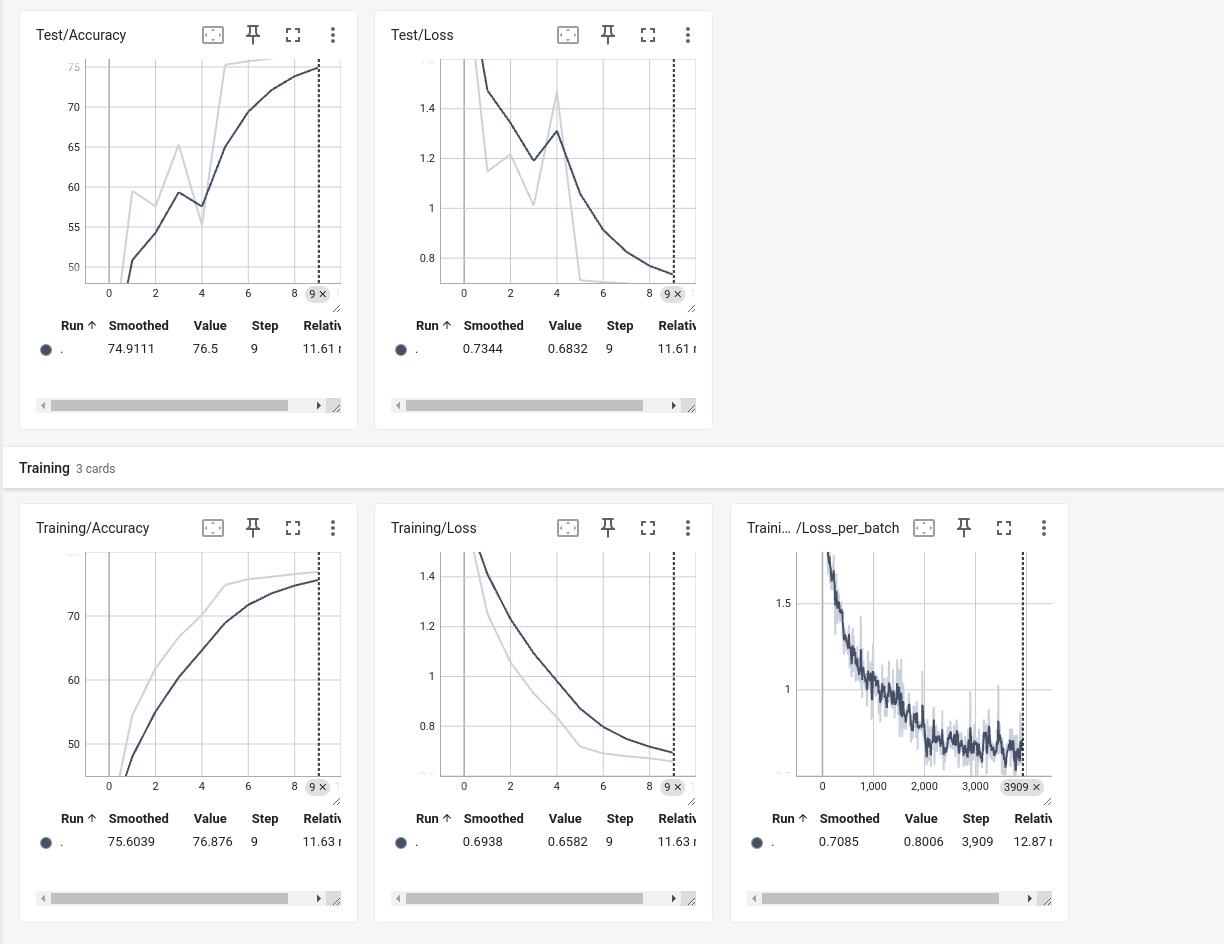
\includegraphics[width=1\textwidth]{./Pytorch/res}
\caption{训练结果}
\end{figure}

    思考题解答:

    Q1: Train acc和Test acc有什么关联和不同?

    A: Train acc是指模型在训练集上的训练正确率,Test acc是指模型在测试集上的正确率。
    通常情况下测试正确率与训练正确率正相关。但当训练次数过多时,可能出现模型在训练集上出
    现过拟合的现象,即在训练集上表现良好,测试集上表现一般。一旦更换同类型的数据,表现会
    变差很多,即缺乏可迁移性。

    Q2: 在lr从0.1变到0.01后,acc发生了什么变化?为什么?

    A: 训练集上的acc波动变小。 对于较大的lr,单次对参数的改变过大,可能出现较理想值略
    大变为较理想值远小的情况,进而导致随训练次数增加,准确率反而下降的情况(如左上图1-2,
    3-4)

\subsection{2.图像特征提取}

    输出日志如下:

\begin{lstlisting}
Extract features!
Time for extracting features: 2.65
The matching result for image 0panda.png
Top 1 similar image : 2.jpeg, with the similarity 99.61307644844055%
Top 2 similar image : 4.jpeg, with the similarity 99.58519339561462%
Top 3 similar image : 5.jpeg, with the similarity 99.58409070968628%
Top 4 similar image : 3.jpeg, with the similarity 99.57888126373291%
Top 5 similar image : 34.jpeg, with the similarity 99.56896305084229%

The matching result for image 1plane.jpeg
Top 1 similar image : 30.jpeg, with the similarity 99.59495067596436%
Top 2 similar image : 8.jpeg, with the similarity 99.5837926864624%
Top 3 similar image : 10.jpeg, with the similarity 99.5837926864624%
Top 4 similar image : 27.jpeg, with the similarity 99.58122968673706%
Top 5 similar image : 35.jpeg, with the similarity 99.57005977630615%

The matching result for image 2lion.jpeg
Top 1 similar image : 5.jpeg, with the similarity 99.56948757171631%
Top 2 similar image : 13.jpeg, with the similarity 99.56185817718506%
Top 3 similar image : 35.jpeg, with the similarity 99.56108331680298%
Top 4 similar image : 50.jpeg, with the similarity 99.55136775970459%
Top 5 similar image : 33.jpeg, with the similarity 99.54777359962463%

The matching result for image 3car.jpeg
Top 1 similar image : 42.jpeg, with the similarity 99.59943294525146%
Top 2 similar image : 18.jpeg, with the similarity 99.57766532897949%
Top 3 similar image : 17.jpeg, with the similarity 99.57575798034668%
Top 4 similar image : 16.jpeg, with the similarity 99.57316517829895%
Top 5 similar image : 44.jpeg, with the similarity 99.56287145614624%

The matching result for image 4train.jpeg
Top 1 similar image : 18.jpeg, with the similarity 99.57295060157776%
Top 2 similar image : 24.jpeg, with the similarity 99.5633602142334%
Top 3 similar image : 35.jpeg, with the similarity 99.5570182800293%
Top 4 similar image : 42.jpeg, with the similarity 99.55503940582275%
Top 5 similar image : 43.jpeg, with the similarity 99.55331683158875%

The matching result for image 5ship.jpeg
Top 1 similar image : 8.jpeg, with the similarity 99.56227540969849%
Top 2 similar image : 10.jpeg, with the similarity 99.56227540969849%
Top 3 similar image : 34.jpeg, with the similarity 99.56071376800537%
Top 4 similar image : 31.jpeg, with the similarity 99.56071376800537%
Top 5 similar image : 30.jpeg, with the similarity 99.55897331237793%

The matching result for image 6chrysanthemum.jpeg
Top 1 similar image : 34.jpeg, with the similarity 99.62146282196045%
Top 2 similar image : 31.jpeg, with the similarity 99.62146282196045%
Top 3 similar image : 32.jpeg, with the similarity 99.59045648574829%
Top 4 similar image : 30.jpeg, with the similarity 99.5827853679657%
Top 5 similar image : 35.jpeg, with the similarity 99.58176612854004%

The matching result for image 7city.jpeg
Top 1 similar image : 39.jpeg, with the similarity 99.6126651763916%
Top 2 similar image : 36.jpeg, with the similarity 99.59376454353333%
Top 3 similar image : 32.jpeg, with the similarity 99.59142208099365%
Top 4 similar image : 33.jpeg, with the similarity 99.56973791122437%
Top 5 similar image : 30.jpeg, with the similarity 99.56700205802917%

The matching result for image 8camera.jpeg
Top 1 similar image : 41.jpeg, with the similarity 99.61915612220764%
Top 2 similar image : 44.jpeg, with the similarity 99.58404302597046%
Top 3 similar image : 45.jpeg, with the similarity 99.56462383270264%
Top 4 similar image : 43.jpeg, with the similarity 99.56437349319458%
Top 5 similar image : 42.jpeg, with the similarity 99.56368207931519%

The matching result for image 9violin.jpeg
Top 1 similar image : 47.jpeg, with the similarity 99.64690208435059%
Top 2 similar image : 48.jpeg, with the similarity 99.63594675064087%
Top 3 similar image : 50.jpeg, with the similarity 99.59607124328613%
Top 4 similar image : 49.jpeg, with the similarity 99.58329796791077%
Top 5 similar image : 46.jpeg, with the similarity 99.57795143127441%

Total Accuracy is 56.0%
\end{lstlisting}

    这里简单认为如果识别到同类别图片则识别正确,否则错误,得到识别正确率为56\%。
    仅使用默认训练参数的情况下,虽然56\%的正确率并不高,但足以接受这个结果。为
    进一步提升匹配正确率,应模仿CIFAR-10构建相应的训练和测试数据进行预训练,再
    进行匹配。考虑数据由手动从网络上下载,数据量不足,不便于实现相关实验。

    通过特征向量的点积结果作为相似度的百分数(和得分),并以此为排序依据,得到每张图和最相似的
    五张图的结果。观察可以发现,照相机(8camera)和小提琴(9violin)组中,
    全部五张同类图像被找到,而在狮子(2lion)、火车(4train)
    和轮船(5ship)组中,仅有一种同类图像被找到。其可能原因在于8、9两组图像特征
    明显且位姿接近,而2、4、5三组存在特征模糊等情况。下面以8组和2组及匹配认为最相近的图像
    为例分析可能的原因(按日志顺序从左至右、从上至下给出,第一张为目标图像)。

\begin{figure}[h]
\centering
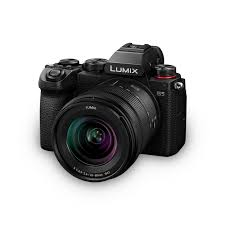
\includegraphics[width=0.28\textwidth]{./CNN/target/8camera}
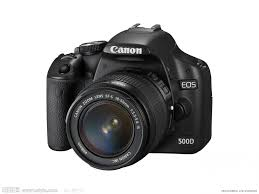
\includegraphics[width=0.28\textwidth]{./CNN/dataset/41}
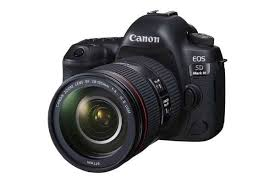
\includegraphics[width=0.28\textwidth]{./CNN/dataset/44}
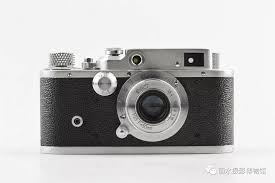
\includegraphics[width=0.28\textwidth]{./CNN/dataset/45}
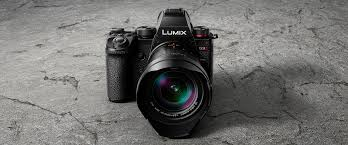
\includegraphics[width=0.28\textwidth]{./CNN/dataset/43}
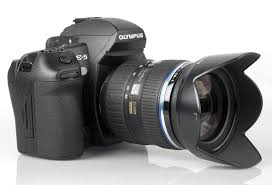
\includegraphics[width=0.28\textwidth]{./CNN/dataset/42}
\caption{第8组结果}
\end{figure}

    第8组中,相机整体由黑色构成,背景以白色居多。在给定数据集中几乎没有
    其他类有如此单调的图像构成。其识别正确率高可以理解。

\begin{figure}[h]
\centering
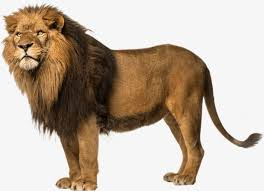
\includegraphics[width=0.28\textwidth]{./CNN/target/2lion}
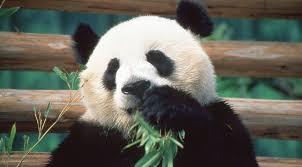
\includegraphics[width=0.28\textwidth]{./CNN/dataset/5}
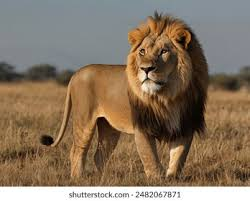
\includegraphics[width=0.28\textwidth]{./CNN/dataset/13}
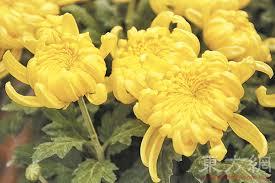
\includegraphics[width=0.28\textwidth]{./CNN/dataset/35}
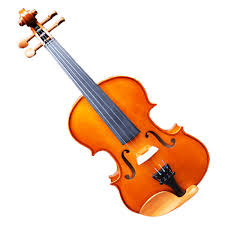
\includegraphics[width=0.28\textwidth]{./CNN/dataset/50}
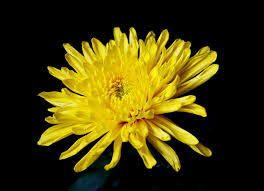
\includegraphics[width=0.28\textwidth]{./CNN/dataset/33}
\caption{第2组结果}
\end{figure}

    第二组中,熊猫背后的栏杆颜色和狮子毛发颜色接近,且有相当的白色构成;
    菊花和小提琴的整体色调也接近狮子,可能导致模型的误判。

\section{实验感想}

    本次实验学习了神经网络检测图像特征的方法,相较于传统方法准确率高且代码实现容易。
    不断调整参数和网络结构也有助于我们对神经网络不同部分的作用有更深入的理解。

\end{document}
